%
% spektral.tex
%
% (c) 2020 Prof Dr Andreas Müller, Hochschule Rapperswil
%
\section{Spektrale Graphentheorie
\label{buch:section:spektrale-graphentheorie}}
\rhead{Spektrale Graphentheorie}
Die Laplace-Matrix codiert alle wesentliche Information eines
ungerichteten Graphen.
Sie operiert auf Vektoren, die für jeden Knoten des Graphen eine
Komponente haben.
Dies eröffnet die Möglichkeit, den Graphen über die linearalgebraischen
Eigenschaften der Laplace-Matrix zu studieren.

\subsection{Grapheigenschaften und Spektrum von $L$
\label{buch:subsection:grapheigenschaften-und-spektrum-von-l}}
TODO XXX 

\subsection{Wärmeleitung auf einem Graphen
\label{buch:subsection:waermeleitung-auf-einem-graphen}}
Die Vektoren, auf denen die Laplace-Matrix operiert, können betrachtet
werden als Funktionen, die jedem Knoten einen Wert zuordnen.
Eine mögliche physikalische Interpretation davon ist die Temperaturverteilung
auf dem Graphen.
Die Kanten zwischen den Knoten erlauben der Wärmeenergie, von einem Knoten
zu einem anderen zu fliessen.
Je grösser die Temperaturdifferenz zwischen zwei Knoten ist, desto
grösser ist der Wärmefluss und desto schneller ändert sich die Temperatur
der beteiligten Knoten.
Die zeitliche Änderung der Temperatur $T_i$ im Knoten $i$ ist proportional
\[
\frac{dT_i}{dt}
=
\sum_{\text{$j$ Nachbar von $i$}} \kappa (T_j-T_i)
=
-
\kappa
\biggl(
d_iT_i
-
\sum_{\text{$j$ Nachbar von $i$}} T_j
\biggr)
\]
Der Term auf der rechten Seite ist genau die Wirkung der 
Laplace-Matrix auf dem Vektor $T$ der Temperaturen:
\begin{equation}
\frac{dT}{dt}
=
-\kappa L T.
\label{buch:graphen:eqn:waermeleitung}
\end{equation}
Der Wärmefluss, der durch die
Wärmeleitungsgleichung~\eqref{buch:graphen:eqn:waermeleitung} beschrieben
wird, codiert ebenfalls wesentliche Informationen über den Graphen.
Je mehr Kanten es zwischen verschiedenen Teilen eines Graphen gibt,
desto schneller findet der Wärmeaustausch zwischen diesen Teilen
statt.
Die Lösungen der Wärmeleitungsgleichung liefern also Informationen 
über den Graphen.

\subsection{Eigenwerte und Eigenvektoren
\label{buch:subsection:ein-zyklischer-graph}}
Die Wärmeleitungsgleichung~\eqref{buch:graphen:eqn:waermeleitung} 
ist eine lineare Differentialgleichung mit konstanten Koeffizienten,
die mit der Matrixexponentialfunktion gelöst werden.
Die Lösung ist
\[
f(t) = e^{-\kappa Lt}f(0).
\]

Die Berechnung der Lösung mit der Matrixexponentialreihe ist ziemlich
ineffizient, da grosse Matrizenprodukte berechnet werden müssen.
Da die Matrix $L$ symmetrisch ist, gibt es eine Basis aus 
orthonormierten Eigenvektoren und die Eigenwerte sind reell.
Wir bezeichnen die Eigenvektoren mit $f_1,\dots,f_n$  und die
zugehörigen Eigenwerte mit $\lambda_i$.
Die Funktion $f_i(t)= e^{-\kappa\lambda_it}f_i$ ist dann eine Lösung
der Wärmeleitungsgleichung, denn die beiden Seiten
\begin{align*}
\frac{d}{dt}f_i(t)
&=
-\kappa\lambda_ie^{-\kappa\lambda_it}f_i
=
-\kappa\lambda_i f_i(t)
\\
-\kappa Lf_i(t)
&=
-\kappa e^{-\kappa\lambda_it} Lf_i
=
-\kappa e^{-\kappa\lambda_it} \lambda_i f_i
=
-\kappa \lambda_i f_i(t)
\end{align*}
von \eqref{buch:graphen:eqn:waermeleitung} stimmen überein.

Eine Lösung der Wärmeleitungsgleichung zu einer beliebigen
Anfangstemperaturverteilung $f$ kann durch Linearkombination aus 
den Lösungen $f_i(t)$ zusammengesetzt werden.
Dazu ist nötig, $f$ aus den Vektoren $f_i$ linear zu kombinieren.
Da aber die $f_i$ orthonormiert sind, ist dies besonders einfach,
die Koeffizienten sind die Skalarprodukte mit den Eigenvektoren:
\[
f=\sum_{i=1}^n \langle f_i,f\rangle f_i.
\]
Daraus kann man die allgmeine Lösungsformel
\begin{equation}
f(t)
=
\sum_{i=1}^n \langle f_i,f\rangle f_i(t)
=
\sum_{i=1}^n \langle f_i,f\rangle e^{-\kappa\lambda_i t}f_i
\label{buch:graphen:eqn:eigloesung}
\end{equation}
ableiten.

\subsection{Beispiel: Ein zyklischer Graph}
\begin{figure}
\centering
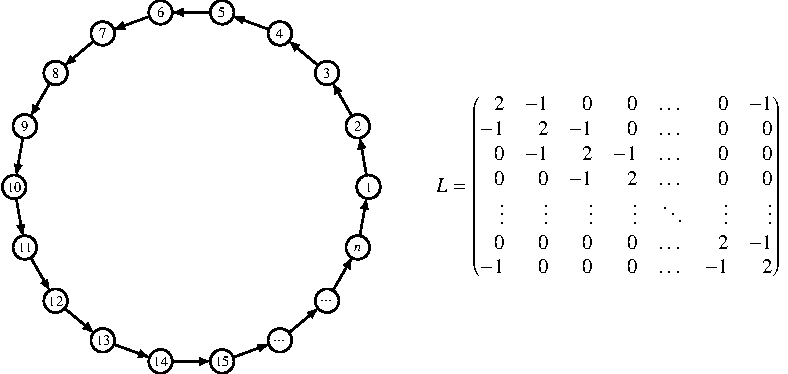
\includegraphics{chapters/70-graphen/images/kreis.pdf}
\caption{Beispiel Graph zur Illustration der verschiedenen Basen auf einem
Graphen.
\label{buch:graphen:fig:kreis}}
\end{figure}
Wir illustrieren die im folgenden entwickelte Theorie an dem Beispielgraphen
von Abbildung~\ref{buch:graphen:fig:kreis}.
Besonders interessant sind die folgenden Funktionen:
\[
\left.
\begin{aligned}
s_m(k)
&=
\sin\frac{2\pi mk}{n}
\\
c_m(k)
&=
\cos\frac{2\pi mk}{n}
\end{aligned}
\;
\right\}
\quad
\Rightarrow
\quad
e_m(k)
=
e^{2\pi imk/n}
=
c_m(k) + is_m(k).
\]
Das Skalarprodukt dieser Funktionen ist
\[
\langle e_m, e_{m'}\rangle
=
\frac1n
\sum_{k=1}^n
\overline{e^{2\pi i km/n}}
e^{2\pi ikm'/n}
=
\frac1n
\sum_{k=1}^n
e^{\frac{2\pi i}{n}(m'-m)k}
=
\delta_{mm'}
\]
Die Funktionen bilden daher eine Orthonormalbasis des Raums der
Funktionen auf $G$.
Wegen $\overline{e_m} = e_{-m}$ folgt, dass für gerade $n$
die Funktionen
\[
c_0, c_1,s_1,c_2,s_2,\dots c_{\frac{n}2-1},c_{\frac{n}2-1},c_{\frac{n}2}
\]
eine orthonormierte Basis.


Die Laplace-Matrix kann mit der folgenden Definition zu einer linearen
Abbildung auf Funktionen auf dem Graphen gemacht werden.
Sei $f\colon V\to \mathbb{R}$ und $L$ die Laplace-Matrix mit
Matrixelementen $l_{vv'}$ wobei $v,v'\in V$ ist.
Dann definieren wir die Funktion $Lf$ durch
\[
(Lf)(v)
=
\sum_{v'\in V} l_{vv'}f(v').
\]

\subsection{Standardbasis und Eigenbasis
\label{buch:subsection:standardbasis-und-eigenbasis}}
Die einfachste Basis, aus der siche Funktionen auf dem Graphen linear
kombinieren lassen, ist die Standardbasis.
Sie hat für jeden Knoten $v$ des Graphen eine Basisfunktion mit den Werten
\[
e_v\colon V\to\mathbb R:v'\mapsto \begin{cases}
1\qquad&v=v'\\
0\qquad&\text{sonst.}
\end{cases}
\]


